\section{Semiotics}
\label{sec:semiotics}

Modern semiotics and linguistics were established in the early 20th century,
mainly influenced by \Person[Charles Sanders]{Peirce} and by
\Person[Ferdinand]{de Saussure} (also named as `semiology'). Influences of both
researchers still exist as independent scholarly traditions. For introductions
to semiotics see \textcite{Eco1976,Eco1977,Eco1984}, \textcite{Chandler2007},
and \textcite{Trabant1996}.  The discipline is related to linguistics, literary
studies, philosophy, cognitive science, and communication science, among other
fields. Some authors have investigated connections between semiotics and
library and information science
\cite{Brier2008,Brier2006,Huang2006,Raber2003,Warner1990,Mai2001}. The
following section briefly introduces to the sign as central concept, justifies
its application to data and digital documents, and highlights some semiotic
results that will assist the phenomenological description of data structuring
and description.

\subsubsection{Digital documents as signs}

The \Term{sign} as core concept of semiotics is most relevant to this thesis.
The classical definition of a sign is often referred to as ``aliquid stat pro
aliquo'' (something stands for something), but this definition has always been
just one component of the function of a sign, even in medieval semiotics
\cite{MeierOeser2011}. More precisely, according to \textcite[paragraph
2.228]{Peirce1931b} a sign is ``something which stands to somebody for
something in some respect or capacity''. The triadic form of Peirce's model of
signs is further described below.  For \textcite{Saussure1916} a sign consists
of a form (\term{signifier}) and a mental concept (\term{signified}) which both
cannot be separated (see figure~\ref{fig:signmodels}). As explained by
\textcite{Taverniers2008}, this dyadic model has been refined by
\textcite{Hjelmslev1953} as relation between expression and content, both
having substance, form and purport among other dimensions.  In the European
tradition the focus of semiotics/semiology later shifted from signs to
signification with researchers such as \Person[Roland]{Barthes}
(\citeyear{Barthes1967}), \Person[Algirdas Julien]{Greimas}
(\citeyear{Greimas1966}),  and \Person[Umberto]{Eco} (\citeyear{Eco1984}).

%, who connect semiotics to
%\term[poststructuralistic]{poststructuralism} positions.

Despite some semiotic focus on linguistic signs (especially words), signs can
also be images, sounds, gestures and other objects, as long as they are
interpreted. Most related to the structuring of description of data there are
approaches to analyse signs in form of diagrams \cite{Bertin2011},
human-computer interaction \cite{Souza2012}, and information
\cite{Brier2008,Huang2006,Raber2003}, but there is no semiotics of data so far.
This thesis includes at least a preliminary semiology of data.  From a semiotic
point of view, a digital document is a sign as soon as it is created or
perceived as document.  In particular it is impossible to create a document
that does not act as some sign, as it is impossible not to communicate
\cite{Watzlawick1967}.  Even an empty file or a random sequence of binary data
can communicate something, for instance the fact that something went wrong.

\subsubsection{Signs are more than signals}

The semiotic view to data as sign reveals some important aspects that are less
visible from other disciplines. First of all, data --- at least if it is given
as some digital document --- is more than a simple signal in the `mathematical
theory of communication'. In this model \cite{Shannon1948} information from a
source is encoded as signal by a sender. The signal is then transmitted to a
receiver and decoded to a destination (see figure~\ref{fig:infosystemmodel}
above and figure~\ref{fig:moody2009fig6} with an illustration of the theory of
communication adopted for diagrams). The information can fully be reconstructed
unless the signal is altered during transmission by noise. In practical data
processing systems this process is nested in chains of encodings and decodings
(figure~\ref{fig:infosystemmodel}).  This model is limited at least for two
reasons. First, the mathematical theory of communication explicitly excludes
all aspects of meaning and it only deals with limited sets of predefined
signals:

\begin{quotation}%
The fundamental problem of
communication is that of reproducing at one point either exactly or
approximately a message \emph{selected} at another point.  Frequently the
messages have meaning; that is they refer to or are correlated according to
some system with certain physical or conceptual entities.  \emph{These semantic
aspects of communication are irrelevant} to the engineering problem. The
significant aspect is that the actual message is \emph{one selected from a set}
of possible messages.\\
\quotationsource \textcite{Shannon1948}, emphasis not included in the original
\end{quotation}

Second, transmitter and receiver are part of the sign. Not only can signals be
changed or interrupted by noise between each encoding and decoding. Also choice
and application of encodings and decoding operations comprises risk of errors.
If data is seen as sign which involves more than simple encoding and decoding,
we can describe nesting by a process of ``unlimited semiosis'' \cite{Eco1979}.
In short, a semiotic sign is not limited to syntax, neither should be digital
documents.

\hfill

\begin{figure}[h]
\centering
\begin{tikzpicture}[font=\sffamily,a/.style={->,very thick},pin edge={a,<-},
c/.style={join=by {a}},mychain/.style={start chain,
every node/.style={align=center,draw,minimum height=5mm}},
ga/.style={a,gray,<-,shorten <=1pt}]

\begin{scope}[node distance=4mm,mychain]
 \node[on chain] {source};
 \node[on chain,c] (e1) {$E_1$};
 \node[on chain,c] (e2) {$E_2$};
 \node[on chain,c,draw=none] (etc) {\ldots};
 \node[on chain,c] (d2) {$D_2$};
 \node[on chain,c] (d1) {$D_1$};
 \node[on chain,c] {destination};
 \node[on chain,draw=none,align=left] 
 	{nested chain of\\encodings/decodings};
\end{scope}

\coordinate (c1) at ($(e1)!.45!(e2)$);
\coordinate (c2) at ($(e2)!.45!(etc)$);
\coordinate (c3) at ($(etc)!.45!(d2)$);
\coordinate (c4) at ($(d2)!.45!(d1)$);

\draw (c1) edge[ga] +(0,+7mm);
\draw (c2) edge[ga] +(0,+7mm);
\draw (etc.center) edge[ga] ++(0,+7mm);
\draw (c3) edge[ga] +(0,+7mm);
\draw (c4) edge[ga] ++(0,+7mm);

\draw[gray,very thick] (c1)+(0,+7mm) edge 
  node[black,fill=white] {noise} ($(c4)+(0,+7mm)$);

\begin{scope}[node distance=6mm,mychain,yshift=15mm]
 \node[on chain] {source};
 \node[on chain,c,label=above:transmitter] {encoding};
 \node[on chain,c,minimum height=3mm,minimum width=3mm,
    pin={below: }] {};
 \node[on chain,c,label=above:receiver] {decoding};
 \node[on chain,c] {destination};
 \node[on chain,draw=none,xshift=-2mm,align=left]
    {communication\\ system};
\end{scope}

\end{tikzpicture}
\caption{Shannon's model of a communication system extended by nesting}
\label{fig:infosystemmodel}
\end{figure}

\pagebreak

\subsubsection{Signs are interpreted}

According to de Saussure, the relationship between signifier and signified is
an \term[arbitrarity]{arbitrary} result of social convention, which is
difficult to change.  The social aspect of signs is relevant also for data: for
instance hyphen, dash, or similar characters can be found to indicate missing
values or not applicable fields, independent from the particular data description
language, but just because of social convention. Data specifications try to
formalize the use of data fields, but all specifications require some social
grounding. 

To better understand how signs are interpreted, it helps to look at
\Person[Charles Sanders]{Peirce}'s triadic model of a sign
(figure~\ref{fig:signmodels}, right).  In this model, a sign is part of an
interaction, which Peirce refers to as \Term{semiosis}. Semiosis involves three
components: the form of a sign
(\Term[representamen|see{symbol}]{representamen}), a mental effect or thought
(\Term[interpretant|see{thought}]{interpretant}), and the thing for which it
stands (\Term[object (semiotic)|see{referent}]{object}).\footnote{Peirce writes
``The thing having this character I term a \emph{representamen}, the mental
effect, or thought, its \emph{interpretant}, the thing for which it stands, its
\emph{object}'' in a in a revised version of a paper from 1867 \cite[paragraph
564]{Peirce1931}. I have not found the original publication of this revision
yet.} This trichotomy can be traced back to \person{Aristotle} and it is also
known as \Term{semiotic triangle} with different names for each of the three
components. Crucial in the semiotic triangle is
the lack of a direct connection between symbol/representamen and
referent/object. A symbol does not stand for a referent, but it is ``used by
someone to stand for a referent'' \cite[p.  11]{Ogden1923}. In practice, the
triadic interaction is embedded in a chain of unlimited semiosis
\cite{Eco1979}: every thought again is a sign in the mind of a person,
interpreted with another thought, and so forth. 

\begin{figure}
\centering
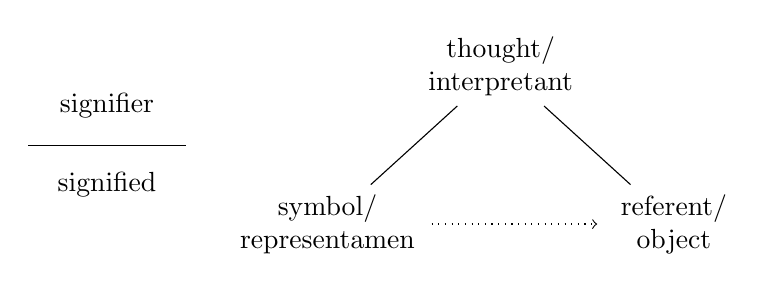
\begin{tikzpicture}
\begin{scope}[xshift=-50mm,yshift=10mm]
\node at (0,5mm) {signifier};
\node at (0,-5mm) {signified};
\draw (-1,0) to (1,0);
\end{scope}
\node[text width=24mm,align=center] at (-22mm,0) (symbol) {symbol/\\representamen};
\node[text width=17mm,align=center] at (22mm,0) (referent) {referent/ object};
\node[text width=20mm,align=center] at (0,2) (thought) {thought/ interpretant};
\draw (symbol) to (thought) (thought) to (referent);
\draw[dotted,->] (symbol) -> (referent);
\end{tikzpicture}
\caption{Dyadic and triadic models of a sign}
\label{fig:signmodels}
\end{figure}

The \term{arbitrarity} of the connection between signifier and signified, based
on social convention, is important to understand that there is no `natural' or
`true' relation between expression and content and that the relation cannot be
derived automatically.  Nevertheless the relation is not random. In addition to
fully arbitrary \Term{symbolic sign}s, Peirce distinguishes \Term{iconic sign}s
with some similarity between symbol and thought (for instance a metaphor or parts
of diagrams as described in section~\ref{sec:diagrams}), and
\Term{indexical sign}s that are directly connected to their thought (for
instance physical traces). This distinction can help at least to explain some
use of data, for instance brackets for grouping and annotation. The
impossibility of automatic derivation neither prevents interpretation of
unknown signs. According to \textcite[section 1.11]{Eco1984} signs are
interpreted by \Term{abduction}. Figure~\ref{fig:reasong} compares abduction
with other methods of logical reasoning: solid boxes indicate known
propositions and dotted boxes indicate tentative propositions produced in the
process of reasoning. Only \Term{deduction} can automatically
\term[inference]{infere} new results by application of formal \term{logic}: for
instance if all objects of type $A$ have some property $B$ (rule) and $a$ is of
type $A$ (case) then $a$ must also have property $B$ (result). Inductive
reasoning reconstructs the meaning of a sign through repeated experiences. If
objects are experienced to have property $B$ every time they are of type $A$,
one may conclude a general rule from these examples. Abduction, in contrast,
directly concludes a rule from a result. In the case of signs, the content is
concluded as as hypothesis from the expression.  For instance if $a$ has some
property $B$, one may presume some type $A$ that is responsible for having $B$.
The abductive diagnosis is often exemplified by detectives which work with
indications.\footnote{The name of William of Baskerville, Eco's main
protagonist in `The name of the Rose', is an allusion to the famous fictional
detective \Person[Sherlock]{Holmes}.} As such, the interpretation of signs is
always tentative and it carries the danger of fallacies: the form of abductive
reasoning is equal to the logical fallacy `post hoc ergo propter hoc' that
takes temporal sequence with casuality.

\begin{figure}
\centering
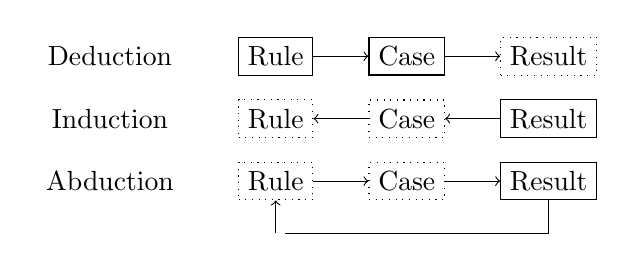
\begin{tikzpicture}
\matrix [column sep=7mm,row sep=3mm,dada/.style={draw,dotted}] {
 \node {Deduction}; & \node(m11)[draw]{Rule};   & \node(m21)[draw]{Case}; & \node(m31)[dada]{Result}; \\
 \node {Induction}; & \node(m12)[dada]{Rule}; & \node(m22)[dada]{Case}; & \node(m32)[draw]{Result}; \\
 \node {Abduction}; & \node(m13)[dada]{Rule}; & \node(m23)[dada]{Case}; & \node(m33)[draw]{Result}; \\
 & \node(m24){}; & \\
};
\draw[->] (m11) to (m21); \draw[->] (m21) to (m31);
\draw[->] (m22) to (m12); \draw[->] (m32) to (m22);
\draw[->] (m13) to (m23); \draw[->] (m23) to (m33);
\draw[->] (m33) |- (m24) -| (m13);
\end{tikzpicture}
\caption{Methods of reasoning, as illustrated by \textcite{Eco1984}}
\label{fig:reasong}
\end{figure}

\subsubsection{Signs are not isolated}

The third result from semiology consists of the fact that signs rarely occur
alone. Instead they are used in a system together with other signs. This system
as described by \person[Charles Sanders]{Peirce} is a language (`langue'), in
contrast to the actual use of a sign in communication (`parole'). The term
language should not be limited to \term[formal language]{formal languages} as
they are described in section~\ref{sec:formallanguages}.  Applied to data as
signs, digital objects do not occur alone, but they are collected and combined
with other digital objects. This collection and combination again is a method
of data structuring. Based on \person[Ferdinand]{e Saussure},
\textcite{Hjelmslev1953} identified syntagm and paradigm as two fundamental
relations by which elements of a language can be connected.

A \Term[syntagm]{syntagmatic} relation consists between elements which occur
together.  An example of syntagmatically connected data elements are \term{file
name}, \term{file type}, and \term{file extension}. Syntagm also provides
context in form of a structure in which elements can be embedded, but syntagm
is not limited to syntax and grammar. Similar elements that can be embedded in
same places are connected by \Term[paradigm]{paradigmatic} relations. Examples
of data elements connected by a paradigmatic relation are arrays and lists, and
the different \acro{RDF} nodes types which can all be used as object in an
\acro{RDF} triple (see table~\ref{tab:rdfvariants}). The final collection of
data patterns (chapter~\ref{ch:patterns}) also includes paradigmatic links
between patterns (as `alternative patterns') and syntagmatic links between
patterns (as `implied`, `specialized` and `related patterns`).

%\Term{paradigm} (from the Greek $\pi \alpha \rho \acute{\alpha} \delta \epsilon \imath
%\gamma \mu \alpha$ for `sample`, `example`, `pattern`) \ldots


\subsubsection{Further insights}

More insights from semiotics and linguistics may be possible if we take into
account the acts of communication which signs are used in. The usual
classification of communication studies includes aspects of \Term{syntax}
(relationships among signs, without reference to their meaning),
\Term{semantics} (relationships between signs and meanings), and
\Term{pragmatics} (relationships between signs and their use). Detailed models
of communication are given for instance by \textcite{Jakobson1963}, in the
theory of \Term{speech acts} \cite{Austin1962,Searle1969}, and in discourse
analysis \cite{Foucault1969}. For the following analysis, however, details of
communication are ignored because our focus is not the situation in which data
is used but the way it is structured and described. Neither does this thesis
include the diachronous nature of data, that is the temporal context in which
it changes. The difference between synchronity and diachronity has also been
introduced by de Saussure, an introduction to this opposition with
application to information as sign is given by \textcite{Raber2003}.

In summary, semiotics provides fruitfull insights to the nature of data, even
with limitation to immutable properties. Taking into account the full nature 
of signs, there are many issues left for further research in data semiotics.

